\chapter{Analyse sécuritaire}
\section{Introduction}
Ce chapitre sur la sécurité a pour but de décrire d'un point de vue sécuritaire le projet élaboré dans le cadre du cours IoT dispensé à la HEIG-VD. Ce dernier est une plateforme de collecte de données environnementales issues de plusieurs capteurs. Dans ce document, les exigences du projet en général seront décrites ainsi que les biens nécessitant une protection contre tout type de menaces ou tout scénarios d'attaque ainsi que les contre-mesures associées. De plus, la liste de tous les composants hardware utilisés pour ce projet est donnée. Toutes les technologies utilisées pour ce projet ont été prises en compte.

\subsection{Equipes}
Lors de ce projet, nous avons créé 5 groupes distincts afin de répartir les différentes compétences et ainsi répartir la charge de travail pour chacun de ces derniers. Chaucun des groupes avaient un répondant pour les autres groupes (représentés en gras ci-dessous).

\renewcommand{\arraystretch}{1.1}
\begin{center}
\begin{tabular}{|l|l|}
	\hline
	Groupe & Etudiant \\
	\hline
	Frontend & \textbf{Aurélie Lévy}  \\
	& Tony Clavien\\
	& Mathias Gilson\\
	\hline
	Backend & \textbf{Ludovic Delafontaine}   \\
	& Guillaume Milani\\
	& Sathiya Kirushnpillai\\
	& Mathieu Monteverde\\
	& Nicolas Rod\\
	& Rodrigue Tchuensu Pouopse\\
	\hline
	Sécurité & \textbf{Lara Chauffoureaux}  \\
	& Matthieu Chatelan  \\
	& Thibaud Besseau  \\
	& Emmanuel Schmid  \\
	\hline
	Firmware & \textbf{David Truan} \\
	& Théo Gallandat\\
	& Gaëtan Othenin-Girard\\
	& Marie Lemdjo\\
	& Ludovic Richard\\
	\hline
	Infrastructure & \textbf{Julien Brêchet} \\
	& Yosra Harbaoui\\
	& Guillaume Semeels\\
	& Adrien Marco\\
	& Ali Miladi\\
	& Dany Tchente\\
	\hline
\end{tabular}
\end{center}
\renewcommand{\arraystretch}{1}

\newpage
\section{Description du système}

\subsection{Objectifs du système}\label{objectifssysteme}% description précise du système (nb de capteurs, leur rôles, infra, ...)

Le but de ce système est la collecte de données depuis plusieurs capteurs répartis sur le site de Cheaseaux. Toutes les informations seront consultables sur un frontend accessible par les visiteurs authentifiés sur un compte publique.

Les différents capteurs (voir \autoref{elementssysteme}) se chargent de récolter des informations relatifs à leur environnement et les transmettent à une gateway dont le but est de collecter ces informations issues des différentes sources. Un bridge assure le lien entre le réseau LoRa et le réseau internet standard. Toutes les informations récoltées sont finalement transmises à un serveur d'applications sur lequel tourne le backend ainsi que le frontend.

Le schéma ci-dessous illustre cette architecture :

\begin{figure}[h!]
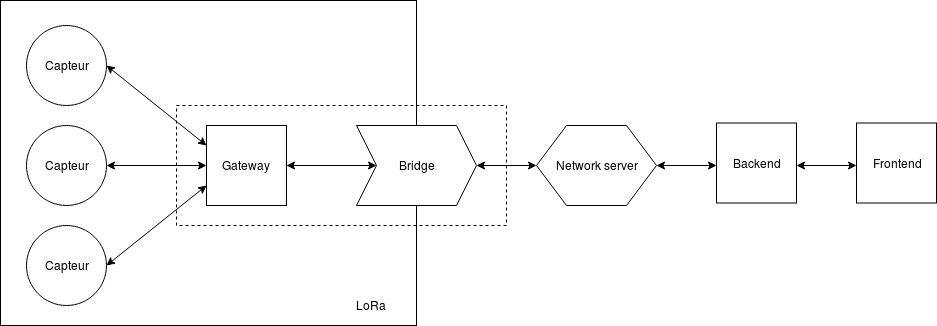
\includegraphics[width=\textwidth]{architecture}
\caption{Schéma de l'architecture du projet}
\end{figure}

\subsection{Exigences de l'application} % Ce qui est nécessaire pour que l'appli fonctionne + au niveau sécu

Pour la sécurité, nous avons interprété les exigences suivantes :

\begin{itemize}
\item[•] L'accès au backend ainsi que l'accès au frontend ne doit être possible que pour les personnes autorisées et authentifiées à l'aide d'un compte que ce soit un compte utilisateur ou administrateur.
\item[•] Un utilisateur classique ne doit pas pouvoir accéder aux fonctionnalités réservées aux administrateurs.
\item[•] Les données transmises par les capteurs ne doivent pas être lisibles sur le réseau.
\end{itemize}

\newpage
\subsection{Éléments du systèmes}\label{elementssysteme} % Les différents capteurs, gateways, etc...

Afin de rendre ce système fonctionnel, plusieurs composants hardware ainsi que software doivent être utilisés. Les sous-sections suivantes représentent les différents modules hardware utilisés ainsi que les parties software développées pour ce projet. Pour chacun des modules hardware, une brève description est donnée (fournie par les fabricants).

\subsubsection{Capteurs}
La carte STM32 Nucleo (\autoref{nucleo}) offre aux utilisateurs un moyen abordable et flexible d'essayer de nouveaux concepts et de construire des prototypes avec le microcontrôleur STM32, en choisissant parmi les différentes combinaisons de performances, de consommation d'énergie et de fonctionnalités. Pour les cartes compatibles, le SMPS réduit considérablement la consommation d'énergie en mode Run.

Cette carte sera utilisée comme base pour tous les capteurs déployés dans le terrain.

\begin{figure}[!h]
	\centering
	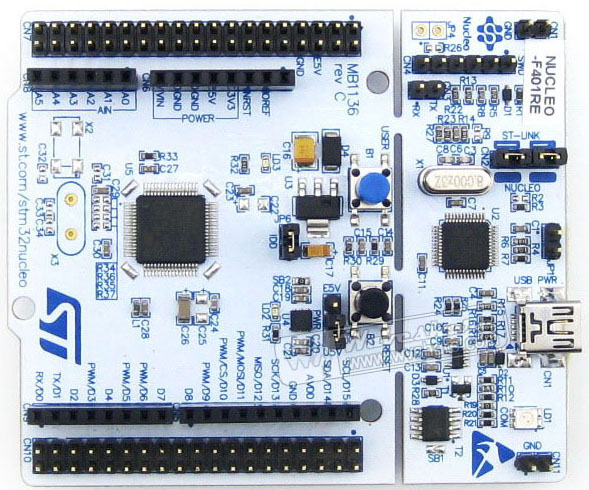
\includegraphics[width=350px]{nucleo}
	\caption{NUCLEO-F401RE}
	\label{nucleo}
\end{figure}

\newpage
Le shield utilisé pour ce projet (\autoref{shield}) rend un Arduino compatible avec plus de 75 capteurs de type clic. C'est un shield simple avec deux prises hôte mikroBUS ™ d'un côté et un connecteur Arduino sur le côté opposé.

\begin{figure}[!h]
	\centering
	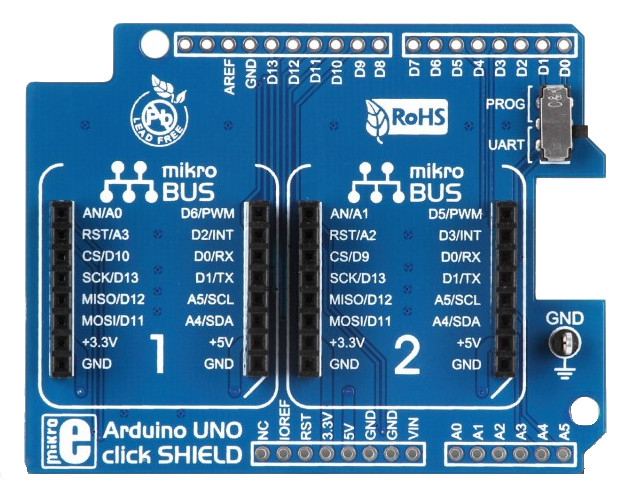
\includegraphics[width=250px]{shield}
	\caption{Arduino Uno Click Shield}
	\label{shield}
\end{figure}

Le module \textit{Environment click} (\autoref{ambient}) mesure la température, l'humidité relative, la pression et les COV (composés organiques volatils gazeux). Le clic intègre le capteur environnemental BME680 de Bosch. L'Environnement Click est conçu pour fonctionner sur une alimentation de 3,3 V. Il communique avec le microcontrôleur cible via l'interface SPI ou I2C.

\begin{figure}[!h]
	\centering
	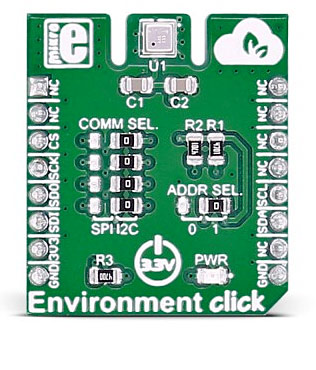
\includegraphics[width=200px]{ambient}
	\caption{Ambient 2 Click BME680}
	\label{ambient}
\end{figure}

\newpage
LoRaWAN ™ ou Low Area Wide Network est une technologie sans fil développée pour permettre des communications à bas débit sur de longues distances, principalement pour les applications IoT et les capteurs.

Le module émetteur-récepteur LoRa longue portée RN2483 de Microchip (\autoref{lora}) est une solution facile à utiliser et à faible consommation d'énergie pour la transmission de données sans fil à longue portée.

Le module RN2483 a une portée spécifiée> 15 km dans les zones rurales et suburbaines, et> 5 km dans les zones urbaines.

Une pile de protocole LoRaWAN ™ classe A est intégrée (périphériques finaux bidirectionnels), ainsi qu'une interface de commande ASCII accessible via UART. La sensibilité élevée du récepteur peut descendre à -148 dBm.
\begin{figure}[!h]
	\centering
	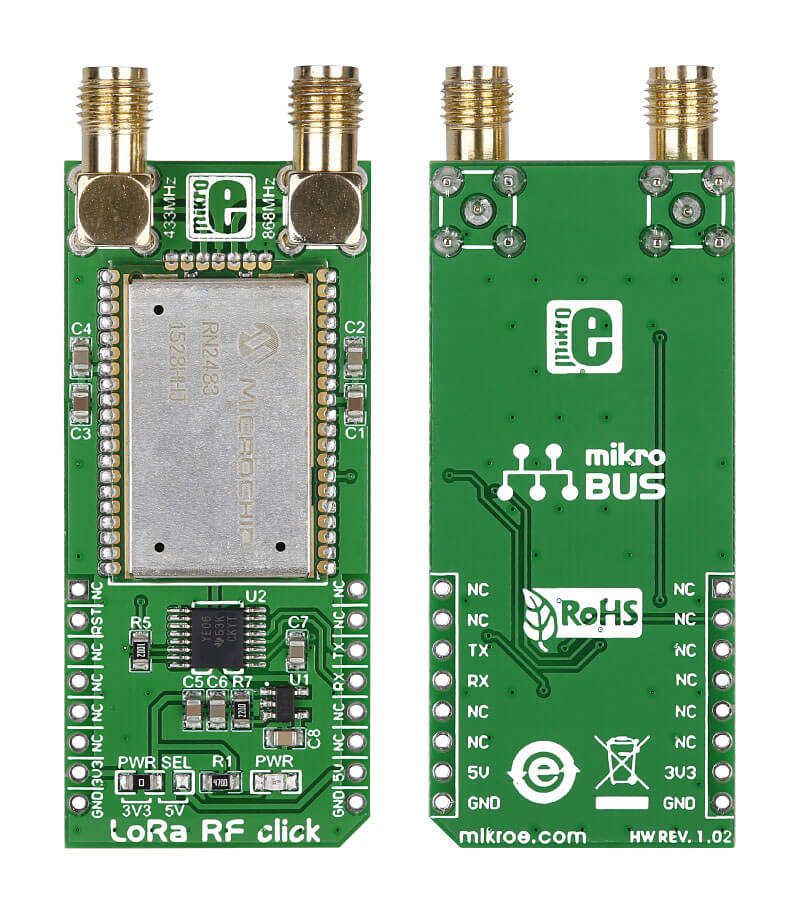
\includegraphics[width=150px]{lora}
	\caption{LoRa Click}
	\label{lora}
\end{figure}

Ci-dessous, une photo du montage complet du capteur avec tous les modules attachés :
\vspace{3mm}
\begin{figure}[!h]
	\centering
	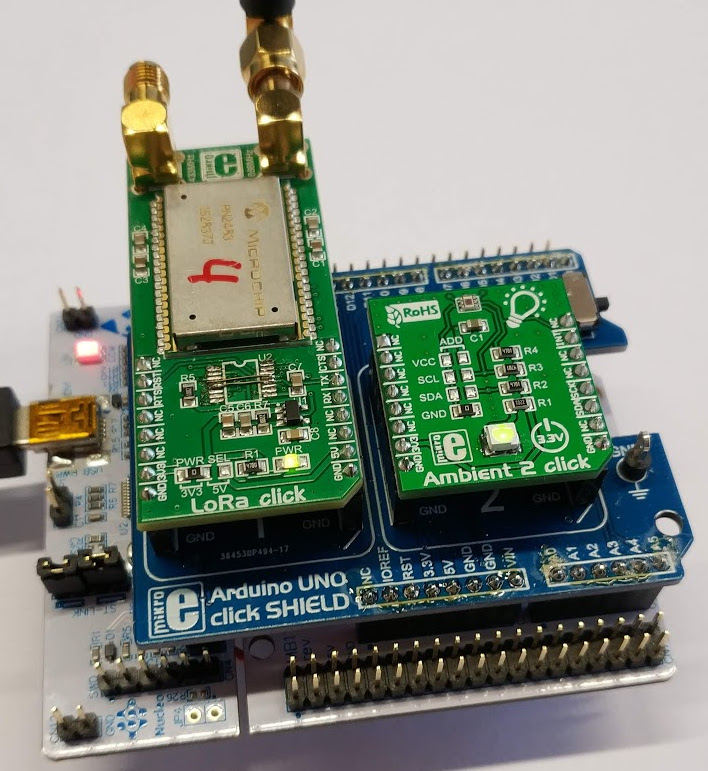
\includegraphics[width=200px]{montage}
	\caption{Montage complet du capteur}
	\label{}
\end{figure}

\newpage
\subsubsection{Gateway}

Le Raspberry Pi 2 Model B est le Raspberry Pi de deuxième génération. Il a remplacé l'original Raspberry Pi 1 Model B+ en février 2015. Ce dernier est utilisé comme base pour la gateway.

Le Raspberry Pi 2 comporte les caractéristiques suivantes :

\begin{itemize}
	\item[•] 900MHz quad-core ARM Cortex-A7 CPU
	\item[•] 1GB RAM
	\item[•] 100 Base Ethernet
	\item[•] 4 Ports USB
	\item[•] 40 pins GPIO
	\item[•] Port HDMI
	\item[•] Jack audio 3.5mm et sortie vidéo composite
	\item[•] Interface Caméra (CSI)
	\item[•] Interface d'affichage (DSI)
	\item[•] Slot pour Micro SD
	\item[•] VideoCore IV 3D coeur graphique
\end{itemize}



\begin{figure}[!h]
	\centering
	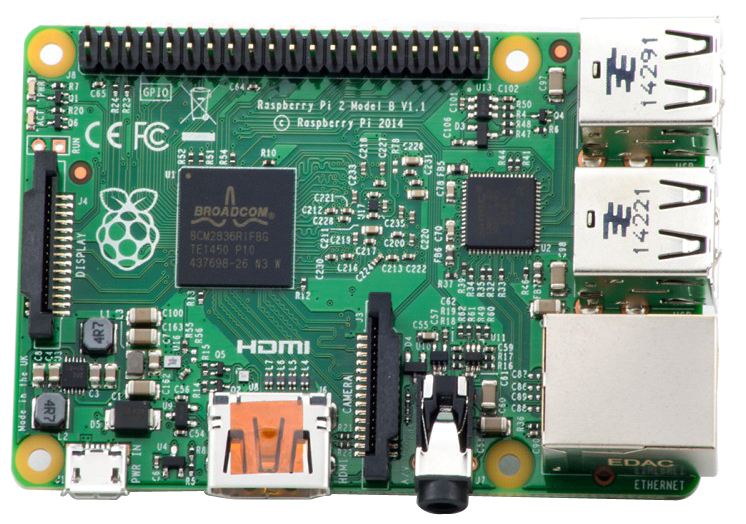
\includegraphics[width=350px]{raspberry}
	\caption{Raspberry Pi Model B}
	\label{raspberry}
\end{figure}

\newpage
Le module iC880A-SPI est capable de recevoir des paquets de différents appareils envoyés avec différents facteurs d'étalement sur jusqu'à 8 canaux en parallèle. En raison du fait que la combinaison des facteurs d'étalement et des largeurs de bande du signal donne des débits de données différents, l'utilisation de "Dynamic Data-Rate Adaption" devient possible. Cela signifie que les nœuds LoRa® à grande distance du concentrateur doivent utiliser des facteurs d'étalement plus élevés et donc avoir un débit de données plus faible.

Les nœuds LoRa qui sont plus proches du concentrateur peuvent utiliser des facteurs d'étalement plus faibles et peuvent donc augmenter leur débit de données. Cela permet de construire des réseaux étoiles ou multi-étoiles faciles à gérer sans besoin de routeurs ou de répéteurs.

\begin{figure}[!h]
	\centering
	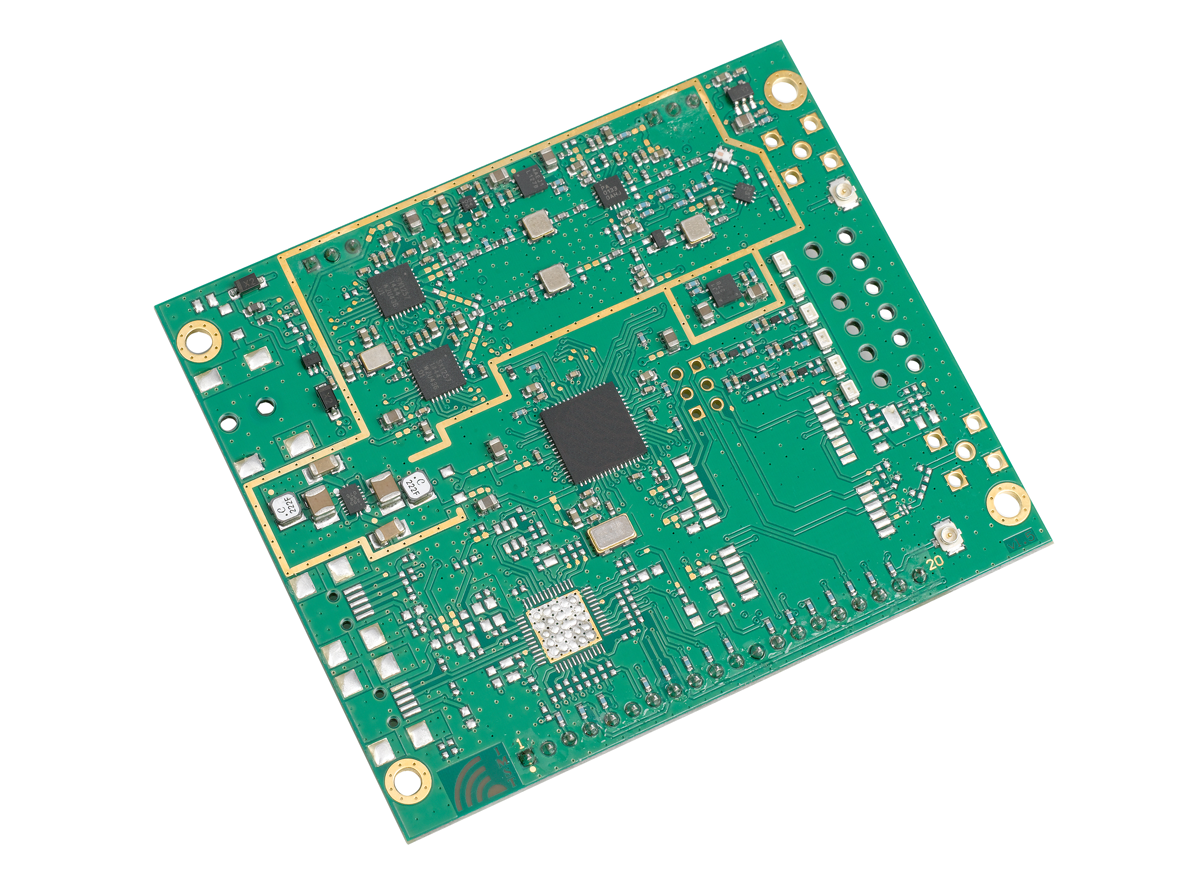
\includegraphics[width=350px]{ic880a-spi}
	\caption{iC880A-SPI - LoRaWAN Concentrator 868 MHz}
	\label{}
\end{figure}

Afin de connecter ce module au Raspberry, un shield tel que le \textit{RPi to iC880a interface} est nécessaire.

\newpage

\subsubsection{Bridge}

Dans notre cas, le bridge fait partie intégrante de la gateway. Sur le schéma dans la \autoref{objectifssysteme}, ce dernier est séparé de la gateway afin de bien représenter le passage de l'utilisation du protocole \textit{LoRa} vers le protocole \textit{MQTT}.
Plus d'informations sont disponibles sur le github suivant : \url{https://github.com/heig-vd-iot2018/infrastructure}

\subsubsection{Network Server}

Ce dernier est divisé en trois parties différentes : Routeur, Broker et Network server.
Plus d'informations sont disponibles sur le github suivant : \url{https://github.com/heig-vd-iot2018/infrastructure}
\subsubsection{Backend}

Le backend est développé en Node.js avec le framework Express. Ce dernier reçoit des informations depuis le network server et traite ces informations avant de pouvoir fournir ces dernières au frontend.
Plus d'informations sont disponibles sur le github suivant : \url{https://github.com/heig-vd-iot2018/back-end}

\subsubsection{Frontend}
Le frontend consiste en la mise en place d'une interface utilisateur permettant de voir les différentes valeurs fournies par les capteurs. Ce dernier a été développé à l'aide des technologies suivantes : \textbf{React}, \textbf{D3} et \textbf{Mapbox.js}.
Plus d'informations sont disponibles sur le github suivant : \url{https://github.com/heig-vd-iot2018/front-end}

%------------------------ Biens a protéger ---------------------------------
\newpage
\subsection{Biens nécessitants une protections}

Les biens principaux à sécuriser sont toutes les données qui peuvent contenir des informations métier ou clients. Par exemple, les données transmises par les capteurs ne doivent pas être lisibles par des personnes non-autorisées au cours de leur trajet sur les différents réseaux empruntés.

Les biens concernés par cette protection sont les suivants :

\begin{itemize}
\item[•] Les données transmises par les capteurs
\begin{itemize}
\item Identité
\item Géo-localisation
\item Données environnementales
\end{itemize}
\item[•] Les données utilisateurs
\begin{itemize}
\item Adresses e-mails \footnote{Afin d'éviter toute réutilisation pour du phishing ou du spamming de masse.}
\item Rôles des utilisateurs \footnote{Pour éviter les vols de session ciblés.}
\item Mots de passe \footnote{Les raisons sont évidentes et de plus ces mots de passe pourraient être ajouté à des listes de brute-force.}
\end{itemize}
\item[•] Le fonctionnement de l'application
\item[•] Les appareils et éléments physiques qui font tourner l'architecture
\end{itemize}

Ces biens doivent être protégés à tous les niveaux et à tous les endroits où elles sont susceptibles d'apparaitre (e.g. des capteurs à la gateway mais aussi de la gateway au serveur d'application).

%------------------------ Périmètre sécurisation ---------------------------
\subsection{Périmètre de sécurisation}

Dans ce projet, la sécurité doit être analysée sur chacun des éléments qui composent l'architecture mais aussi sur les liens entre eux. Il n'y a aucune zone considérée comme "sûre de base", il faut donc penser à tous les éléments suivants :

\begin{itemize}
\item[•] Sécurisation des connexions aux éléments physiques.
\item[•] Sécurisation des trames à l'intérieur du protocole LoRa.
\item[•] Sécurisation des accès au back-end et au front-end.
\item[•] Sécurisation de toutes les communications MQTT.
\item[•] Sécurisation des éléments hébergeant les différents éléments de l'infrastructure.
\item[•] Sécurisation et gestion des version pour les technologies, langages et librairies utilisées.
\end{itemize}
\clearpage

%------------------------ Diagramme des flux -------------------------------
\subsection{Diagramme des flux}
\label{ssec:diagramme}

\begin{figure}[h!]
\centering
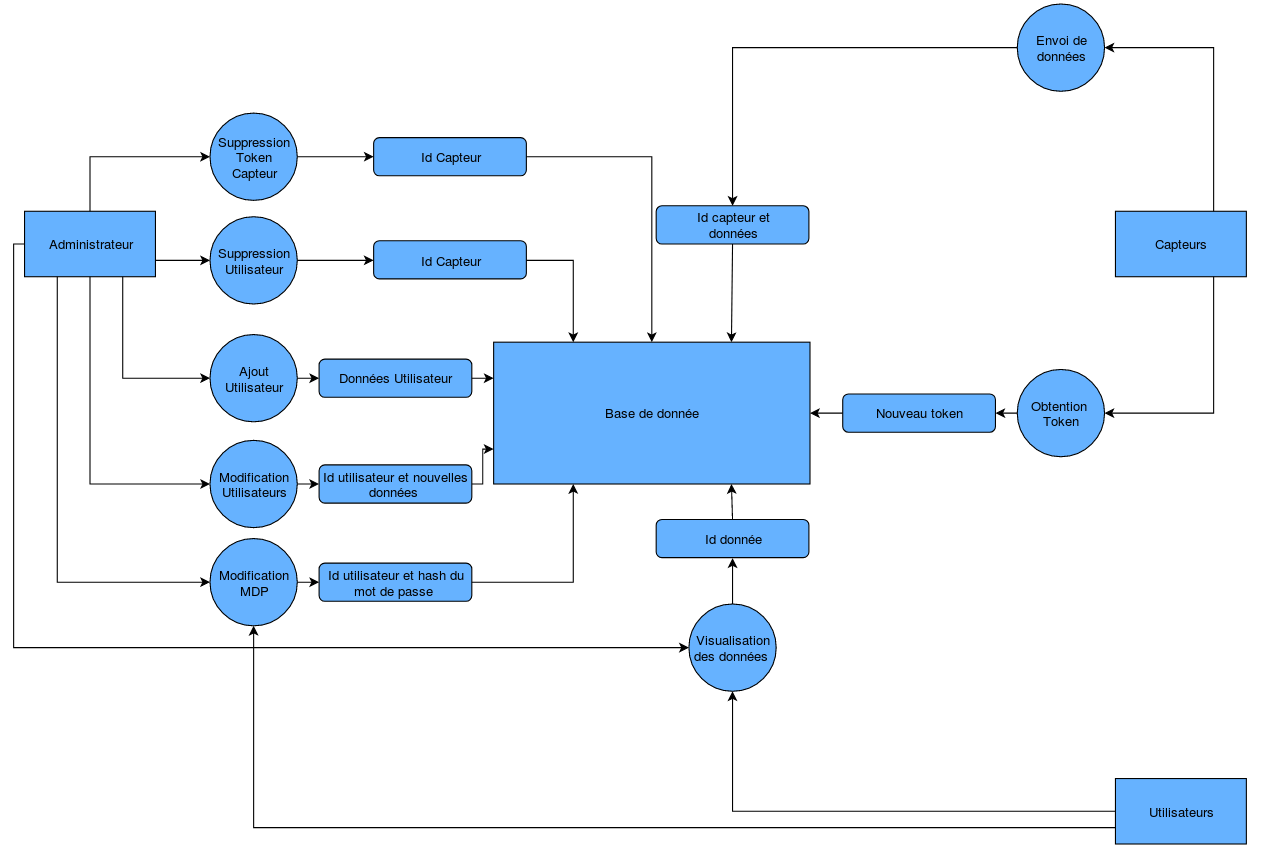
\includegraphics[angle=90, width=.85\textwidth]{diagramme_flux}
\caption{Diagramme des flux}
\end{figure}

%------------------------ Sources de menaces -------------------------------
\clearpage
\section{Sources de menaces}

Différentes sources de menaces existent autour des applications web mais aussi autour du monde de l'\emph{Internet des objets}. Dans le cadre de notre projet nous retrouvons les catégories de menaces décrites ci-dessous :

\begin{itemize}

\item[•] \textbf{Étudiants kleptomanes}

\begin{tabular}{lp{13cm}}
Motivation: & Gagner un capteur, une gateway, une Raspberry Pi gratuite \\
Cible: & Le matériel \\
Probabilité: & Haute \\
\end{tabular}
\medskip

\item[•] \textbf{Hacker, script-kiddies}

\begin{tabular}{lp{13cm}}
Motivation: & S'amuser, s'entraîner, le faire pour la reconnaissance \\
Cible: & Tout ce qui peut être visé et qui entre dans ses compétences \\
Probabilité: & Moyenne \\
\end{tabular}
\medskip

\item[•] \textbf{Éventuels concurrents}

\begin{tabular}{lp{13cm}}
Motivation: & Récupération des particularités de l'application (espionnage industriel) \\
Cible: & Le fonctionnement de l'application \\
Probabilité: & Moyenne \\
\end{tabular}
\medskip

\item[•] \textbf{Cybercriminels}

\begin{tabular}{lp{13cm}}
Motivation: & Récupérer des adresses mails (spaming) et mots de passe, se servir de l'application web comme passerelle vers son site malveillant ou pour répandre un virus \\
Cible: & Les données des utilisateurs, l'accès à la partie web \\
Probabilité: & Faible \\
\end{tabular}
\medskip

\item[•] \textbf{Organisation étatique}

\begin{tabular}{lp{13cm}}
Motivation: & Récolter des données, espionner \\
Cible: & Toute l'application \\
Probabilité: & Presque nulle \\
\end{tabular}
\medskip

\end{itemize}
\newpage

%------------------------ Début scénarios ----------------------------------
\section{Scénarios d'attaque}
\label{sec:scenarios}

Dans les sections ci-dessous, différents scénarios d'attaque sont listés et analysé en détails. Pour chacun d'eux, les failles qui existaient dans le projet ont été listées et analysées. Toutes les contre-mesures applicables pour les corriger sont détaillées dans la \autoref{sec:contremesures}. Dans la \hyperref[sec:conclusion]{conclusion}, vous retrouverez toutes les listes des failles existantes, absente, corrigées ou exploitables.

Un scénario d'attaque correspond à une marche à suivre qu'un attaquant souhaitant attaquer le système suivrait pour arriver à ses fins. Celui-ci est généralement élaboré par un ingénieur sécurité s'étant mis à la place d'un attaquant. Cet exercice permet de mieux comprendre les vecteurs d'attaque, l'impact, les motivations et les potentielles cibles d'un individu malveillant. Ces scénarios ne représentent pas les failles sécuritaires à proprement parler, mais les motivations générales qu'un attaquant peut avoir pour attaquer le système.

Chacun des chapitres ci-dessous reprend donc un scénario d'attaque ainsi que les failles qui lui sont associées. Avec chaque scénario, se trouve un résumé des enjeux et la liste des failles ainsi que la manière dont elles peuvent être exploitées.

\subsection{Vol d'informations dans la base de données}

\emph{Ce scénario concerne principalement les groupes front-end et back-end}.
\medskip

Comme dans la plupart des applications web et des projets de cette envergure, le groupe \emph{back-end} a mis en place une base de données. Celle-ci est évidemment une cible privilégiée pour les attaquants car elle contient toutes les informations métiers et celles nécessaires à la plateforme web.
\medskip

\renewcommand{\arraystretch}{1.6}
\begin{tabular}{@{}p{4cm}p{12cm}}
\textbf{Scénario:} &  Un hacker décidé à récupérer des données pour son nouveau dictionnaire de mots de passe suisses romands, connaît l'existence d'un jeune projet à la HEIG-VD. En accédant au site web, il découvre une vulnérabilité lui permettant de récupérer les données présentes dans la base de données. Il peut donc compléter son dictionnaire qu'il utilisera à des fins malveillantes. \\
\textbf{Impact:} & Moyen \\
\textbf{Source de menace: } & Concurrents, script kiddies, hackers et cybercriminels \\
\textbf{Motivation:} & La gloire (script kiddies, hackers)

L'argent (cybercriminels)

L'espionnage industriel (concurrents) \\
\textbf{Cible:} & Données utilisateurs et données métier \\
\textbf{Contrôles:} & Caché le contenu de la base de données

Sécuriser son accès
\end{tabular}
\renewcommand{\arraystretch}{1}

\subsubsection{Injections NoSQL}

Quand on parle de failles touchant les bases de données, on pense forcément au numéro 1 du top 10 de l'OWASP : les injections SQL. Dans notre application, la base de données déployée n'est pas une base de données SQL mais MongoDB. Néanmoins, après quelques recherches sur Google, on apprend vite que cela ne change rien et que de telles failles existent aussi en NoSQL. L'existence d'une telle faille dans le système mènerait au scénario décrit ci-dessus du vol de données. Voici le lien officiel de l'OWASP expliquant en gros le fonctionnement et la détections de telles injections dans un base de données MongoDB :

\url{https://www.owasp.org/index.php/Testing_for_NoSQL_injection}

Une courte explication des contre-mesures envisageables pour une telle faille est donnée dans la \autoref{ssec:cm-injections}

\subsubsection{Lisibilité du contenu sensible}

Ceci ne reprend pas vraiment une faille à proprement parler mais plutôt une précaution qu'il faut prendre lors du développement d'une application web. Imaginons que nous ayons corrigés les failles permettant les injections NoSQL décrites ci-dessus, mais qu'une faille zero-day soit découverte sur les librairies utilisées par notre application. Malgré nos protections mises en place, un attaquant pourra donc accéder au contenu de la base de données et récupérer les mots de passe et autres données confidentielles.

Prévenir vaut mieux que guérir et donc chiffrer et saler les mots de passe dans la base de données s'avère nécessaire. Cela permet d'éviter que les sessions utilisateurs soient compromises sans aucune attaque par dictionnaire ou par brute-force.

Dans les contremesures, une explications plus poussée du salage et du hachage sont données. Voici néanmoins les conseils de l'OWASP à ce propos : \url{https://www.owasp.org/index.php/Password_Storage_Cheat_Sheet}

\subsubsection{Configuration de la base de données}

La configuration d'une base de données est très importante car de nombreux points peuvent vite s'avérer cruciaux en cas d'attaque :

\begin{itemize}
\item[•] Si une base de données n'est pas maintenue à jour, elle peut être la cible d'attaques diverses et connues sur les versions antérieures. \href{https://www.cvedetails.com/vulnerability-list/vendor_id-12752/product_id-25450/Mongodb-Mongodb.html}{Une liste longue comme le bras de vulnérabilités} existe sur les anciennes versions de MongoDB. Il est donc essentiel de garder la base de données à jour.
\item[•] Une mauvaise gestion de droits des utilisateurs de la base de données peut être dangereux si un utilisateur accède directement à la base données.
\item[•] Une notion importante dans une base de données est celle de \emph{built-in function}. En cas de réussite d'une attaque NoSQL, si celle-ci sont laissées activées par défaut, le pivot et la compromission complète de la base de données devient facile pour un attaquant même inexpérimenté.
\end{itemize}

Les contre-mesure de la \autoref{ssec:cm-configdb} expliquent quels modèles utiliser pour la configuration d'une telle base de données.

%\begin{itemize}
%\item Injections SQL
%\item Conservation des mots de passe dans la DB
%\item Accès direct à la base de données (port 3306 ouvert)
%\item Gestion version, droits utilisateurs, built-in fonctions
%\end{itemize}

\clearpage
\subsection{Contournement d'authentification}

\emph{Ce scénario concerne principalement les groupes front-end et back-end}.
\medskip

Comme précisé dans notre diagramme des flux (\autoref{ssec:diagramme}), nous voyons qu'il existe plusieurs rôles communiquant avec le back-end.

\begin{enumerate}
\item Les administrateurs
\item Les utilisateurs normaux
\item Les capteurs
\end{enumerate}

Ceux-ci disposent bien évidemment de possibilités différentes dans le cadre du projet. Évidemment cette séparation des pouvoirs est importante et les cloisonnement des rôles est primordial afin de limiter au maximum les abus. Un utilisateur normal ayant la possibilité d'abuser le système pour devenir administrateur, peut représenter un grand risque pour la plateforme. Tous les autres cas de changement illicite de rôle sont tout aussi risqués et il est nécessaire de mettre en place des protections contre ce genre de motivations.
\medskip

\renewcommand{\arraystretch}{1.6}
\begin{tabular}{@{}p{4cm}p{12cm}}
\textbf{Scénario:} &  Jean-Kevin, un script kiddy entreprenant, souhaite montré à ses copains ses progrès en informatique. Pour cela, il prend pour cible un projet sur lequel travaille activement un de ces collègues étudiant à la HEIG-VD. Il veut montrer qu'il peut se connecter en tant qu'administrateur sans connaître le
mot de passe. Il arrive à ses fins en se connectant au compte d'un
administrateur qui n'était pas protéger par un mot de passe fort et
peut disposer à sa guise de l'application.\\
\textbf{Impact:} & Haut \\
\textbf{Source de menace: } & Script kiddies, hackers \\
\textbf{Motivation:} & La gloire (script kiddies)

Nuire à l'application et aux utilisateurs (hackers)\\
\textbf{Cible:} & Données et fonctionnement de l'application \\
\textbf{Contrôles:} & Protéger la session ouverte contre des vols de sessions externes

Empêcher l'utilisateur de faire malgré lui des actions dans sa session

Protéger correctement les sessions avec des mots de passe forts
\end{tabular}
\renewcommand{\arraystretch}{1}

\subsubsection{Cross-site scripting}

Une faille XSS exploitée correctement par un attaquant permet de voler un cookie de session valide ou de faire en sorte que du code soit exécuté involontairement par un utilisateur. Cette vulnérabilité fait aussi partie du top 10 de l'OWASP.

Voici le lien officiel décrivant donc le fonctionnement de telles attaques :

\url{https://www.owasp.org/index.php/Top_10-2017_A7-Cross-Site_Scripting_(XSS)}

\subsubsection{Brute-force du système de login}

Une autre possibilité pour réaliser ce scénario est la brute force pur et simple du système de login. Sans contrôle particulier, un utilisateur possédant un bon dictionnaire de nom d'utilisateurs et de mots de
passe peut tenter de forcer le login de l'application et donc d'accéder directement à une session qui n'est pas la sienne.

\subsubsection{\emph{Cross-site request forgery}}

Les attaques CSRF \footnote{Petit rappel sur le CSRF : \url{https://en.wikipedia.org/wiki/Cross-site_request_forgery}} sont souvent ignorée dans les applications web et pourtant, elles peuvent avoir des conséquences importantes au niveau de la sécurité. Une faille CSRF est difficile à
mettre en évidence et à exploiter, mais si aucune protection n'a explicitement été mise en place, on peut supposer que l'application en question sera vulnérable aux CSRF.

\subsubsection{Contrôles d'accès}

Le contrôle d'accès est un point \textbf{crucial} de la sécurité des applications web. Si un utilisateur lambda peut accéder à une page ou à une fonction administrateur, l'aboutissement du scénario est complet. Si le contrôle d'accès n'est pas bien fait, une élévation verticale ou horizontale des privilèges devient possible.

Rappelons ici que notre application possède quatre vues en tout :

\begin{itemize}
\item[•] Les simples visiteurs non-connectés
\item[•] Les utilisateurs standards
\item[•] Les administrateurs
\item[•] Les capteurs
\end{itemize}

Le contrôle d'accès doit bien évidemment \textbf{cloisonner} chacun des rôles à sa propre vue même si les implications ne semblent pas importantes. Pour cela, la \autoref{ssec:cm-controleacces} de contremesures décrit un système qui peut être implémenté pour un contrôle d'accès correct avec une structure comme la notre.

\subsubsection{Durée de vie de la session}

Si l'application ne vérifie pas la durée de vie d'une session. Un utilisateur laissant sa session connectée  laisserait n'importe quelle personne qui, prenant la main sur l'ordinateur, utiliser le compte de l'utilisateur.
Prenons l'exemple de l'utilisateur allant chercher un café. Si une personne avait accès à l'ordinateur de l'utilisateur il pourrait faire toutes les opérations qu'il voudrait avec ce compte pendant une durée illimitée. De plus, si celui-ci est un peu doué en informatique, il peut copier le cookie de session pour le réutiliser à volonté depuis son ordinateur.

En cas de ban d'un utilisateur, le manque de durée de vie est aussi problématique. Imaginons qu'un administrateur décide de bannir un utilisateur en supprimant son compte. Si cet utilisateur est connecté au moment du bannissement, il n'aura aucune répercussion à part s'il perd son cookie, ce qui est assez rare. Tandis qu'avec une durée de vie de session, ce dernier, après un certain temps, ne pourra plus effectuer d'action sur le site et sera déconnecté.

%\begin{itemize}
%\item XSS
%\item Brute-force login
%\item CSRF et autres
%\item Contrôle d'accès
%\item Durée de vie de session
%\end{itemize}

\subsection{Récupération passive d'information}

\emph{Ce scénario concerne principalement le groupe infrastructure.}
\medskip

Souvent, on imagine un hacker pénétrant le système et réalisant des \textbf{actions} sur ce dernier. Ne considérer que ce pan de la sécurité est une grave méprise. Rappelons le triangle suivant :

\begin{figure}[h]
\begin{center}
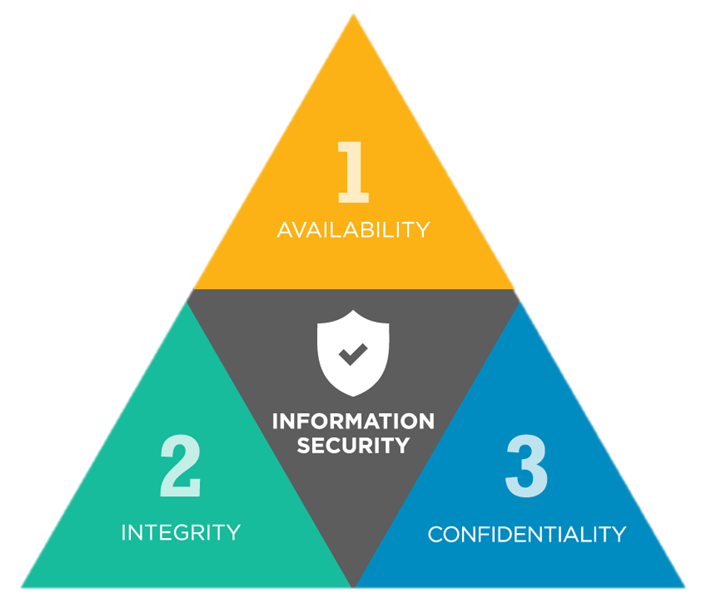
\includegraphics[width=.6\textwidth]{CAI.png}
\label{cia}
\caption{Principes essentiels de la sécurité informatique}
\end{center}
\end{figure}

La confidentialité peut en effet être mise à mal sans même une action directe sur les données. L'interception de données peut permettre la lecture de ces dernières et si l'information n'est pas obfusquée, on peut récupérer des données sans le consentement des parties et donc mettre à mal la sécurité de l'information. Il est donc primordial de protéger les données dans leur transmission surtout sur des médiums partagés tels que les réseaux sans fils.
\medskip

\renewcommand{\arraystretch}{1.6}
\begin{tabular}{@{}p{4cm}p{12cm}}
\textbf{Scénario:} &  Les concurrents directs de notre application cherche à obtenir un maximum de données afin de proposer un service plus précis et exhaustif que le notre. Pour arriver à leur fins ils décident d'écouter le trafic généré par nos capteurs à l'intérieur de l'école. Si le trafic n'est pas chiffré, les concurrents peuvent l'utiliser de manière illicite dans leur alternative.\\
\textbf{Impact:} & Haut \\
\textbf{Source de menace: } & Hackers, concurrents et cybercriminels \\
\textbf{Motivation:} & Tremplin vers une plus grosse attaque (hackers)

L'argent (cybercriminels)

Nuire à notre image, voler des données (concurrents)\\
\textbf{Cible:} & Les données utilisateurs et métier \\
\textbf{Contrôles:} & Éviter que l'application ne fournisse des données sur elle-même ou sur les utilisateurs

Protéger les communications entre les éléments du système
\end{tabular}
\renewcommand{\arraystretch}{1}

\subsubsection{Communications en clair}

Le wifi est une chose fantastique, mais malheureusement les données passent dans l'air et donc tout le monde peut les "voir". Cela implique évidemment que toutes les données passent en clair sur le réseau mots de passe et données comprises. C'est évidemment pas sécurisé et la confidentialité des données est fortement impactée. Le compromis idéal est la mise en place d'un tunnel TLS pour toutes les communications HTTP de notre projet. Plus de détails sur la mise en place d'un tel système sont donnés dans la \autoref{ssec:cm-tls}.

Le protocole HTTP classique n'est pas le seul utilisé dans notre projet. Nous utilisons aussi le protocole LoRa qu'il faut donc aussi rendre illisible pour toute personne effectuant une capture sur le réseau.

\subsubsection{Messages d'erreur révélant des informations}

Les messages d'erreur sont un moyen de communiquer comme un autre avec l'utilisateur. Il ne doivent en aucun cas révéler des informations qui pourraient être exploitées par quelqu'un de malveillant.

L'exemple le plus courant est celui du message d'erreur au login indiquant si oui ou non un utilisateur existe. Cela donne déjà beaucoup d'information à un hacker qui n'aura plus qu'à deviner le mot de passe pour usurper la session.
\clearpage
%\begin{itemize}
%\item SSL/TLS
%\item Chiffrement des trames LoRa
%\item Messages d'erreurs
%\end{itemize}

\subsection{Utilisation frauduleuse du matériel}

\emph{Ce scénario concerne principalement le groupe firmware.}
\medskip

La nature d'un projet en Internet des Objets implique la présence de capteurs et ou autres éléments physiques dans un bâtiment. Évidemment ces éléments sont exposés "au public" et peuvent être pris pour cibles par des personnes mal-intentionnées. Cette partie de la sécurité est important mais aussi relativement difficile à mettre en place.
\medskip

\renewcommand{\arraystretch}{1.6}
\begin{tabular}{@{}p{4cm}p{12cm}}
\textbf{Scénario:} &  Un étudiant un peu curieux et kleptomane sur les bords repère dans l'école une jolie borne composée d'une Raspberry Pi. Celui-ci décide un jour que la borne ne sert pas à grand chose et il l'embarque pour son usage personnel.\\
\textbf{Impact:} & Haut \\
\textbf{Source de menace: } & Étudiants kleptomanes, script-kiddies \\
\textbf{Motivation:} & Profit personnel (étudiants kleptomanes)

La gloire (script-kiddies)\\
\textbf{Cible:} & Le matériel et le fonctionnement de l'application \\
\textbf{Contrôles:} & Ne pas laisse le matériel à des endroits accessibles à tous

Mettre en place des "fuse protections" sur les éléments physiques
\end{tabular}
\renewcommand{\arraystretch}{1}

\subsubsection{Accès non-contrôlé au hardware}

Empêcher le vol du matériel est quelque chose de compliqué parce que c'est une mesure qui pourra toujours être contournée avec des moyens. Si le concepteur met le dispositif dans un boite, la boite peut être volée etc...

Pourtant c'est un point qu'il est important de ne pas négliger dans un projet pareil car le matériel coûte cher.

\subsubsection{Composants réinscriptibles}

Au cas où le matériel aurait été subtilisé malgré les protections mises en place au point précédent, il faut éviter au maximum que le profiteur ait envie de recommencer. Si celui-ci vole du matériel et peut être en mesure de l'utiliser, ça peut vivement l'encourager à recommencer. Alors que si des protections sont mises en place, le risque est un peu mitigé. Dans les contre-mesures de la \autoref{ssec:cm-fuse}, une méthode très connue des développeurs hardware est présentée pour protéger les matériaux contre un écrasement de leur contenu actuel.
\clearpage

%\begin{itemize}
%\item Protection modification du hardware (signature, tamper-proofing)
%\item Contrôle d'accès physique
%\item Association sécurisée
%\end{itemize}

\subsection{Altération des données}

\emph{Ce scénario concerne principalement les groupes infrastructure et firmware.}
\medskip

D'ordinaire, on se dit qu'un individu malveillant cherche forcément à avoir le contrôle complet de sa cible. Néanmoins, le plus souvent un contrôle ou une altération partielle du système ou des données peut avoir de grosses conséquences sur le système. Il est donc très important de protéger dans les trois axes présentés précédemment dans la \autoref{cia} : confidentialité, intégrité, disponibilité.
\medskip

\renewcommand{\arraystretch}{1.6}
\begin{tabular}{@{}p{4cm}p{12cm}}
\textbf{Scénario:} &  Un concurrent direct à notre application désire montrer que leur solution est meilleure que la notre. Pour cela, ils décident d'altérer les données transmises par nos capteurs pour qu'elles soient erronées. Plusieurs endroits peuvent être vulnérables notamment les trames LoRa et les données transmises par le back-end. Il faut être capable d'éviter des attaques de type \emph{man in the middle}.  \\
\textbf{Impact:} & Moyen \\
\textbf{Source de menace: } & Concurrents, hackers, organisations étatiques \\
\textbf{Motivation:} & Nuire à l'image de l'entreprise (concurrents)

L'argent (hackers)

L'espionnage (organisations étatiques)\\
\textbf{Cible:} & Les données métiers\\
\textbf{Contrôles:} & Contrôle d'intégrité sur les données transmises

Contrôle de l'association capteurs - serveur
\end{tabular}
\renewcommand{\arraystretch}{1}

\subsubsection{\emph{Man in the middle}}

Les attaques de types \emph{man in the middle} (MITM) sont très connues. Les attaquants font en sorte, lors d'une attaque de ce type, de se retrouver comme intermédiaire entre deux éléments du système. D'un coté le client aura l'impression de converser avec le bon serveur et le serveur avec un client légitime.

Pour limiter ce type d'attaque, on utilise les contrôles d'intégrité mis sur les trames. Ceux-ci reviennent à signer les messages avec une clé privée afin que ceux-ci ne puissent être modifié par un MITM sans que cela ne se répercute sur la signature. Dans notre cas, il conviendra de protéger les communications HTTP (avec TLS par exemple), et les communications LoRa.

Plus de détails sur ces contre-mesures sont documentée dans les sections \ref{ssec:cm-tls} et \ref{ssec:cm-mitm}.

\subsubsection{Association des capteurs à la passerelle}

Pour un individu malveillant, un moment idéal pour réaliser une attaque \emph{man in the middle} est celui ou les composants s'associent. Le moment où un capteur est ajouté au système est crucial car c'est là que le lien de confiance est établi. Des précautions particulières sont a apporter sur ce point, et des protocoles existants du LoRa permettent cette association avec sécurité.

%\begin{itemize}
%\item Signature des trames LoRa
%\item \emph{Man in the middle}
%\item Association sécurisée (capteur - serveur)
%\end{itemize}

\subsection{Altération du fonctionnement de l'application}

\emph{Ce scénario concerne la plupart des groupes.}
\medskip

De nos jours, les données sont la cible privilégiée des attaques. Néanmoins, une altération ou une interruption du service est tout aussi dommageable pour l'entreprise. Une perte de confiance des utilisateurs nuit rapidement à la réputation et à l'image du prestataire de service. Des fois les hackers jouent sur ce tableau afin de se faire de l'argent facilement sur le dos des entrepreneurs. C'est un problème sécuritaire majeur dans les systèmes et tous les pans du projet peuvent être vulnérables. Ce scénarios reprend en vrac toutes les attaques qui peuvent affecter la disponibilité et le fonctionnement de l'application.
\medskip

\renewcommand{\arraystretch}{1.6}
\begin{tabular}{@{}p{4cm}p{12cm}}
\textbf{Scénario:} &  Une organisation de cybercriminels cherche une nouvelle cible et tombe par hasard sur notre projet. Pour se faire de l'argent ils décident de compromettre l'application en la ralentissant ou en touchant sa disponibilité tout en faisant des demandes de rançon aux concepteurs. \\
\textbf{Impact:} & Moyen \\
\textbf{Source de menace: } & Concurrents, script-kiddies, hackers \\
\textbf{Motivation:} & Nuire à l'image de l'entreprise (concurrents)

L'argent (hackers)

La gloire (script-kiddies)\\
\textbf{Cible:} & La disponibilité, le fonctionnement de l'application\\
\textbf{Contrôles:} & Redondance des éléments

Contrôle des entrées utilisateurs
\end{tabular}
\renewcommand{\arraystretch}{1}

\subsubsection{Attaque par déni de service}

Tous les systèmes informatiques quels qu'ils soient sont vulnérables aux dénis de service. Le principe reste très simple : envoyer trop de requêtes / demandes / trames à une entité pour que celle-ci devienne incapable de toutes les traiter et soit ralentie voir arrêtée. Le problème principal du DDoS (\emph{Distributed Denial of Service}), est qu'il n'est pas possible à endiguer entièrement même avec toutes les mesures du monde. Une menace disposant de moyen techniques et financiers illimités sera toujours capable de créer un dénis de service sur une cible.

Néanmoins nous présentons dans la \autoref{ssec:cm-ddos} plusieurs moyen de mitiger un peu les risques. Mais il convient de garder à l'esprit que pour le dénis de service la protection ultime n'existe pas.

\subsubsection{Brouillage du réseau}

Une autre attaque qu'il est difficile voir impossible de contrer et le brouillage réseau. Nous n'allons pas plus en parler ici car c'est un risque qui pèse sur tout le monde des ondes hertziennes et qui ne peut pas être mitigé à cause des législation qui régissent les réseaux sans-fil (bandes ISM, puissance isotrope rayonnée équivalente).

\subsubsection{Intrusion dans les systèmes hébergeurs}

Malgré toute les failles multiples et variées que nous avons traitées jusqu'ici, l'essentiel pour les hackers reste l'intrusion généralisée et classique dans un système. Un port ouvert avec un service vulnérable, une version de l'OS dépassée comportant des failles de sécurité et des failles permettant une escalade de privilège vers un compte administrateur de la machine et \textbf{tout le système est compromis dans l'arrière boutique}.

Ces attaque sont les plus dangereuses car elles donnent un accès complet à tous les services, à tous les fichiers, à toutes les bases de données, à toutes les clés privées utilisées pour mettre en place la sécurité jusqu'ici. De plus un attaquant disposant d'un tel contrôle sur une machine d'hébergement peut purement et simplement supprimer le service, l'application, le projet ou même formater complétement tout ce qui lui passe sous la main.  Évidemment, inutile de parler de l'impact immense qu'une telle attaque peut avoir sur un système.

\subsubsection{Ralentissement volontaire de la base de données}

Il ne faut jamais faire confiance à un utilisateur, jamais. Toutes les entrées doivent être contrôlées lors du développement d'un tel projet. Que ce soit pour éviter les attaques de type injection NoSQL ou XSS mais aussi pour éviter une surcharge de données pouvant mener à un ralentissement d'une base de données.

Par exemple un champ beaucoup trop grand ~1'000'000 de caractères représente environ 1 MB de données à stocker dans une base de données. Si l'abus est répété, on arrive vite à un volume de données important qui peut ralentir considérablement une base de données (même NoSQL !).
\clearpage

%------------------------ Contremesures ------------------------------------
\section{Contre-mesures}
\label{sec:contremesures}

Comme nous avons dans ce projet beaucoup de scénarios, de failles et donc de contre-mesures, nous n'allons donc pas les développer en détails ici. Néanmoins, pour chacune d'entre elle un descriptif plus ou moins fourni de la technique est donné. Celui-ci est accompagné de liens \footnote{En anglais, car la bonne documentation est en anglais} vers des solutions existantes pour une architecture proche de notre système.

Il est à noter que les contre-mesures doivent, dans la mesure du possible, utiliser des librairies existantes et considérées comme sécurisées et à jour. Les solutions \emph{"home made"} sont à éviter car généralement elles vont souffrir de manquements ou d'oublis.

\subsection{Injection NoSQL}
\label{ssec:cm-injections}

Pour protéger notre base de données de ce type d'attaque, il faudrait nettoyer les entrées de toutes lignes de codes exécutables. Pour ce faire, il faudrait utiliser la librairie suivante : mongo-sanitize.

Le code ci-dessous donne un example de quand utiliser cette librairie (source \href{https://www.npmjs.com/package/mongo-sanitize}{NPM}):
\vspace{2mm}
\begin{lstlisting}[style=Java]
var sanitize = require('mongo-sanitize');

var name = sanitize(req.params.name);
var password = sanitize(req.params.password);

User.findOne({ "name" : name, "password" : password }, callback);
\end{lstlisting}

\medskip
\textbf{Librairies et documentation :}

\begin{itemize}
\item[•] \href{https://www.npmjs.com/package/mongo-sanitize}{Outil -- Librairie NPM de mongo-sanitize}
\item[•] \href{https://zanon.io/posts/nosql-injection-in-mongodb}{Article -- Injection NoSQL dans Node avec MongoDB}
\item[•] \href{https://stackoverflow.com/questions/13436467/javascript-nosql-injection-prevention-in-mongodb}{Stackoverflow -- Injection prevention in MongoDB}
\item[•] \href{https://www.owasp.org/index.php/Testing_for_NoSQL_injection}{OWASP -- Testing for NoSQL injection}
\end{itemize}

\subsection{Lisibilité du contenu sensible}
\label{ssec:cm-hash}

Afin de protéger les mots de passe des utilisateurs même en cas de vol de la base de données, il est indispensable de hacher les mots de passe avec des méthodes de hachages qualifiés de surs comme SHA256 ou SHA3. Ainsi, même en ayant tous les hashs des utilisateurs, l'attaquant n'a pas les mots de passe des utilisateurs et ne peut donc pas utiliser leurs comptes.

Afin d'augmenter encore la sécurité de notre application, nous pouvons ajouter du sel à notre application. Le sel consiste à concaténer au mot de passe de l'utilisateur une chaine de caractère aléatoire afin que deux mots de passe identiques ne donnent pas le même hash. Cette chaine de caractère est stockée dans la base de données. Le sel est une excellente protection contre les attaques par rainbow table car il faut brute forcer les mots de passe un par un.
\clearpage

\medskip
\textbf{Librairies et documentation :}

\begin{itemize}
\item[•] \href{https://www.owasp.org/index.php/Password_Storage_Cheat_Sheet}{OWASP -- Password storage cheatsheet}
\item[•] \href{https://stackoverflow.com/questions/6951563/storing-passwords-with-node-js-and-mongodb}{Stackoverflow -- Storing passwords with Node.js and MongoDB}
\item[•] \href{https://github.com/kelektiv/node.bcrypt.js}{Outil -- Bcrypt pour Node.js}
\item[•] \href{https://www.abeautifulsite.net/hashing-passwords-with-nodejs-and-bcrypt}{Article -- Node et bycrypt}
\end{itemize}

\subsection{Configuration de la base de données}
\label{ssec:cm-configdb}

Afin de sécuriser notre base de données NoSQL, l'idéal serait de définir les rôles selon un modèle RBAC (Role based Access Control).

Ainsi, chaque compte de la base de données ne donnera accès qu'aux fonctions dont a besoin le service ou l'utilisateur. Il faut aussi logger les accès à la base de données afin de pouvoir détecter d'éventuels comportements suspects ou bugs. De plus pour assurer une bonne disponibilité de cette BDD, il faudrait la monitorer pour pouvoir détecter les problèmes en amont.

Si la tolérance au down time pour notre application venait à devenir critique, nous devrions envisager de mettre en place un système de base de données redondant. Il serait aussi nécessaire de définir une politique de backup afin de pouvoir se prémunir contre une perte ou une altération de nos données.

\medskip
\textbf{Librairies et documentation :}

\begin{itemize}
\item[•] \href{https://docs.mongodb.com/manual/core/authorization/}{Documentation officielle -- RBAC dans MongoDB}
\item[•] \href{https://docs.mongodb.com/manual/tutorial/manage-users-and-roles/}{Documentation officielle -- Gestion des utilisateurs et des rôles}
\item[•] \href{https://docs.mongodb.com/manual/administration/security-checklist/}{Documentation officielle -- MongoDB security checklist}
\end{itemize}

\subsection{\emph{Cross-site scripting}}
\label{ssec:cm-xss}

Pour protéger notre application contre les attaques de type xss, il faudrait passer les entrées fournit par l'utilisateur dans un filtre choisi afin d'échapper correctement tout code malveillant.

\medskip
\textbf{Librairies et documentation :}

\begin{itemize}
\item[•] \href{https://www.owasp.org/index.php/XSS_(Cross_Site_Scripting)_Prevention_Cheat_Sheet}{OWASP -- XSS prevention cheat sheet}
\item[•] \href{http://scottksmith.com/blog/2015/06/22/secure-node-apps-against-owasp-top-10-cross-site-scripting/}{Article -- XSS et applications Node.js}
\item[•] \href{https://www.npmjs.com/package/xss}{Outil -- Librairie NPM de xss nettoyage des inputs}
\item[•] \href{https://www.npmjs.com/package/secure-filters}{Outil -- Librairie NPM de secure-filters nettoyage des inputs}
\end{itemize}

Plein d'autres librairies existantes et correctes sont disponibles dans Node.js !
\clearpage

\subsection{Brute-force du système de login}
\label{ssec:cm-bruteforce}

Afin de se protéger contre les attaques de type brute force ou envoi massif de formulaire, il faudrait mettre des captchas (comme les reCAPTCHAS de Google) afin de s'assurer que c'est bien un humain qui effectue l'action. Ainsi on rendrait impossible les attaques de type brute force effectuées à l'aide de scripts. De plus, le reCAPTCHAS de Google est vraiment simple d'utilisation et gère de manière automatique une blacklist des adresses IP qui ont tenté de brute-forcer un formulaire.

\medskip
\textbf{Librairies et documentation :}

\begin{itemize}
\item[•] \href{https://www.google.com/recaptcha/intro/v3beta.html}{Documentation officielle -- Google reCAPTCHA}
\item[•] \href{https://codeforgeek.com/2016/03/google-recaptcha-node-js-tutorial/}{Turoriel -- Google reCAPTCHA avec Node.js}
\item[•] \href{https://www.npmjs.com/package/express-recaptcha}{Outil -- Librairie NPM de express-recaptcha}
\item[•] \href{https://www.npmjs.com/package/recaptcha2}{Outil -- Librairie NPM de recaptcha2}
\end{itemize}

\subsection{\emph{Cross-site request forgery}}
\label{ssec:cm-csrf}

La contre-mesures la plus répandu pour se protéger des failles web de type CSRF est l'authentification par token. Lorsqu'une requête est soumise au serveur, un header supplémentaire contenant le token est ajouté. Le token est vérifié avant de réaliser l'action. La génération du token est une étape critique. Il est nécessaire qu'il soit généré de manière aléatoire, n'utilisant que des librairies standards.

Il existe d'autres contre-mesures additionnelles, notamment ajouter des étapes de validation (confirmation, captcha) lors des actions jugées critiques. Optionnellement, il est possible de vérifier depuis quelle page la requête a été effectuée. Bien qu'une contre-mesure supplémentaire ne soit pas de refus, il faut savoir qu'il est possible de forger une requête et donc de modifier cette valeur.

\medskip
\textbf{Librairies et documentation :}

Voir la documentation de la contre-mesure contrôle d'accès dans la \autoref{ssec:cm-controleacces}.

\subsection{Contrôle d'accès}
\label{ssec:cm-controleacces}

Il est légitime de contrôler l'accès aux différentes parties de l'application afin de s'assurer que l'utilisateur possède les autorisations nécessaires pour accéder à l'information. Le contrôle d'accès prend la forme d'une page de login. Une fois authentifié, l'utilisateur doit recevoir en retour un \emph{Json Web Token} par exemple. Il s'agit d'une technologie très utilisée dans les back-end Javascript. Ce token est envoyé à chaque requête de l'utilisateur. Il contient diverses informations :
\begin{itemize}
\item[•] Rôle
\item[•] Date d'émission
\item[•] Signature
\item[•] Émetteur
\item[•] Etc...
\end{itemize}
\medskip

Si le token est valide \textbf{(vérification de la signature)} et n'est pas blacklisté dans une base de donnée, alors la session reste active. Ce type de token empêche à un attaquant de déterminer l'identifiant de session de quelqu'un et donc d'usurper son identité.

\medskip
\textbf{Librairies et documentation :}

\begin{itemize}
\item[•] \href{https://jwt.io/}{Documentation officielle -- Json Web Token}
\item[•] \href{https://www.npmjs.com/package/jsonwebtoken}{Outil -- Librairie NPM de jsonwebtoken}
\item[•] \href{https://tools.ietf.org/html/rfc7519}{Norme -- Json Web Token}
\end{itemize}

\subsection{Durée de vie de la session}
\label{ssec:cm-dureeviesession}

La durée de vie d'une session dépend des informations et des actions dont l'utilisateur a besoin. Il est important de trouver un juste milieu; si la durée de vie est trop courte, alors l'utilisateur sera obligé de s'authentifier plusieurs fois par jour. Dans le cas contraire, l'inattention d'un utilisateur quittant son bureau sans verrouiller sa session, permettrait à un collègue d'accéder à son compte pendant son absence. De plus, les actions et les données auxquelles un utilisateur standard ou un administrateur à accès sont différentes. C'est pourquoi une distinction entre ces 2 types de profils est nécessaires.

\begin{description}
\item[Utilisateur] 10 jours
\item[Administrateur] 1 jour
\end{description}

En plus de cette distinction et de cette durée de vie, il convient d'avoir une base de données permettant de stocker les tokens correspondant à une session black-listée ou bannie. Pour cela, une simple collection MongoDB de tokens suffit amplement si on pense à la vérifier après chaque vérification de JWT.

\medskip
\textbf{Librairies et documentation :}

\begin{itemize}
\item[•] \href{https://www.owasp.org/index.php/Session_Management_Cheat_Sheet#Session_ID_Life_Cycle}{OWASP -- Session management cheat sheet}
\item[•] Toute la documentation de la contre-mesure \ref{ssec:cm-controleacces} sur les Json Web Token.
\end{itemize}

\subsection{Communication en clair}
\label{ssec:cm-tls}

\subsubsection{LoRa}

Pour des questions de confidentialité des données, les trames ne peuvent pas circuler en clair sur le réseau. Il suffirait à un attaquant de sniffer le réseau pour avoir accès aux informations. Cette contre-mesure est implémentée de base par LoRaWAN.

\subsubsection{Certificat SSL pour serveur nginx}

Afin de chiffrer les communications entre nos clients et notre serveur web nginx.
Pour cela, nous avons créé un \texttt{dockerCompose} qui nous permet de créer un serveur nginx proxy, un serveur nginx et un serveur \emph{nginx let's encrypt compagnion}.
\medskip

\begin{itemize}

\item[•] \textbf{Nginx Proxy}
\vspace{1mm}

Notre serveur proxy nginx aura pour tâche de centraliser toutes les requêtes HTTPS et de les rediriger vers les serveurs adéquats (dans notre cas, vu que nous avons qu'un seul service web toutes les requêtes seront redirigées vers notre service nginx).
Vu que notre proxy est accessible directement depuis internet, il possède un certificat SSL délivré par Let's Encrypt.
Ce certificat est renouvelé à intervalle régulière par le container \emph{nginx let's encrypt compagnion}
\vspace{3mm}

\item[•] \textbf{\emph{Nginx let's encrypt compagnion}}
\vspace{1mm}

Ce container se réveille périodiquement (une fois par heure) et vérifie que le certificat du proxy nginx est toujours valable et qu'il n'expire pas dans moins de 30 jours.
Si le certificat est valide et que sa durée de validité est supérieure à 30 jours, il se rendort pour une heure.
Dans le cas où le certificat serait absent, invalide ou expirerait dans moins de 30 jours, le container en régénère un et le place dans le dossier certificats du proxy nginx et se rendort pour une heure.
\vspace{3mm}

\item[•] \textbf{Serveur nginx}
\vspace{1mm}

Ce container est notre serveur web, il reçoit les requêtes des clients que lui transmet le proxy et lui renvoie le contenu demandé par les clients.
\end{itemize}

\medskip
\textbf{Librairies et documentation :}

\begin{itemize}
\item[•] \href{https://meta.discourse.org/t/help-multisite-with-letsencrypt-nginx-proxy-companion/88192}{Article -- Gestion multi-site avec nginx et let's encrypt}
\item[•] \href{https://github.com/JrCs/docker-letsencrypt-nginx-proxy-companion}{Outil -- Image Docker Hub \texttt{JrCs/docker-letsencrypt-nginx-proxy-companion}}
\item[•] \href{https://github.com/jwilder/nginx-proxy}{Outil -- Image Docker Hub \texttt{jwilder/nginx-proxy}}
\item[•] \href{https://hub.docker.com/_/nginx/}{Outil -- Image Docker Hub \texttt{nginx}}
\item[•] \href{https://labs.mwrinfosecurity.com/assets/BlogFiles/mwri-LoRa-security-guide-1.2-2016-03-22.pdf}{Guide -- LoRa security}
\end{itemize}

\subsection{Messages d'erreur révélant des informations}
\label{ssec:cm-messageserreurs}

Nos messages d'erreur sur notre version en production doivent donner le minimum d'informations. Par exemple en cas d'erreur de notre serveur nginx celui-ci doit seulement donner le numéro et le type d'erreur. En aucun cas, il ne doit donner la cause de cette erreur car le message indiquant la cause pourrait divulguer certaines informations utiles à un attaquant. De même, notre serveur nginx ne devra jamais fournir son numéro de build dans un message d'erreur car il suffirait à un attaquant de chercher sur internet les failles pour la version de notre serveur.

Un autre endroit où les messages d'erreur doivent être le plus vague possible est le login. Le message d'erreur en cas de saisie de mauvais identifiants ne doit pas dire si le compte existe ou ce qui est faux entre le nom d'utilisateur et le mot de passe. Il devra juste donner un message générique comme celui-ci: "La connexion a échoué. Veuillez vérifier vos identifiants".

\medskip
\textbf{Librairies et documentation :}

\begin{itemize}
\item[•] \href{https://www.owasp.org/index.php/Error_Handling}{OWASP -- Error handling}
\item[•] \href{https://cwe.mitre.org/data/definitions/209.html}{MITRE-CWE 209 -- Information exposure through an error message}
\end{itemize}

\subsection{Accès non-contrôlé au hardware}
\label{ssec:cm-acceshardware}

L'accès aux différents modules (gateway et capteurs) doit être protégé afin d'éviter à une tierce partie d'accéder au firmware ou programmes qui tournent sur ces derniers. En effet, si des clés de chiffrement sont disponible sur ces modules afin de chiffrer les trames envoyées entre les senseurs et les gateway, il faut s'assurer que l'accès à cette information soit protégé.

Il serait envisageable, comme première mesure, d'enfermer ces modules dans des armoires techniques fermées à clé afin d'en limiter l'accès.

\subsection{Composants réinscriptibles}
\label{ssec:cm-fuse}

Afin de garantir la persistance du hardware en cas de vol, les constructeur ont mis en place un système appelé "fuse protection". Ces "protection fuse" peuvent être de type logiciel ou matériel. Ils permettent d'éviter que les éléments de la mémoire soient lus, et par conséquent, sont de plus en plus installés dans les chips de nos jours. Cette protection est mise en place, par exemple, en configurant certains bits dans le chip ou en fusionnant les lignes de contrôle correspondantes. Ces \textit{fuse} ne sont pas toujours résistants à différentes techniques de manipulation spécifiques. Ces \textit{Fuse bits} qui sont configurés peuvent être remis à 0 par une injection par laser. Une fois que ces \textit{fuse} sont remis à 0, l'analyse du système (lecture des informations) peut continuer. Une contremesure efficace est un maillage de connecteurs qui est placé autour du chip et qui est électriquement connecté à ce dernier. Si le chip est ouvert ou attaqué physiquement, ce maillage est détruit ce qui résulte en la destruction du chip, rendant impossible la récupération des informations (voir \autoref{laser}).

\begin{figure}[!h]
	\centering
	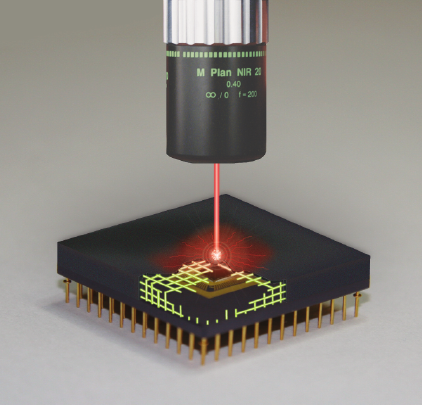
\includegraphics[width=250px]{laserattack.png}
	\caption{Protection anti-modification par maillage}
	\label{laser}
\end{figure}

\medskip
\textbf{Librairies et documentation :}

\begin{itemize}
\item[•] \href{https://www.aisec.fraunhofer.de/content/dam/aisec/Dokumente/Publikationen/Studien_TechReports/englisch/Whitepaper_ProductProtection.pdf}{Article -- Protecting embedded systems against product piracy}
\end{itemize}

\subsection{\emph{Man in the middle}}
\label{ssec:cm-mitm}

Afin de garantir l'intégrité des données envoyées sur le réseau LoRa, un contrôle d'intégrité de type CRC32 peut être effectué à l'instar du type de contrôle effectué lors de communications Wifi. Cette somme de contrôle serait mise à la suite des données envoyées et le tout pourrait être chiffré, par exemple avec AES dont la clé serait connue du capteur et de la gateway.

Une fois la trame reçue par la gateway, ou par le capteur, elle serait déchiffrée et le CRC32 contrôlé afin d'assurer l'intégrité de la trame reçue.

\medskip
\textbf{Librairies et documentation :}

\begin{itemize}
\item[•] \href{https://www.owasp.org/index.php/Man-in-the-middle_attack}{OWASP -- Man in the middle attack}
\item[•] Toute la documentation de la contre-mesure \ref{ssec:cm-tls} sur le chiffrement des communications et les tunnels TLS.
\end{itemize}

\subsection{Association des capteurs à la passerelle}
\label{ssec:cm-association}

La sécurité du réseau LoRaWAN repose sur deux chiffrements AES-128.

\begin{itemize}
\item[•] \textbf{Network Session Key} (NwkSKey) assure l'authenticité des nœuds du réseau. La \emph{NwkSKey} permet à l'opérateur de sécuriser le réseau. Cette clé est connue par l'opérateur du réseau et par les fournisseurs d'applications autorisés.
\item[•] \textbf{Application Session Key} (AppSKey) assure la confidentialité des données. La \emph{AppSKey} permet au fournisseur de l'application de protéger les données transitant par le réseau. Cette clé n'est connue que du fournisseur de l'application. Aucun service tiers peut donc déchiffrer le contenu des messages.
\end{itemize}

Les données envoyées sont chiffrées avec la \emph{AppSKey} et un en-tête est ajouté. Cet en-tête contient notamment les adresses source et destination. Sur la base de cette nouvelle donnée, un MIC est calculé à l'aide de la \emph{NwkSKey}  pour garantir l'intégrité. Ce MIC permet au réseau de vérifier l'intégrité du message et authentifier le nœud de l'envoie.

\subsubsection{Activation}

Les équipements souhaitant communiquer sur le réseau LoraWAN doivent premièrement obtenir des clés de sessions. Deux méthodes sont disponibles : \textbf{Over-The-Air Activation} (OTAA) ou \textbf{Activation By Personalization} (APB) qui est hors scope dans notre cas.

Le nœud doit transmettre une \emph{join request} au réseau sur la base de 3 paramètres.
\begin{enumerate}
\item Un identifiant unique (type EUI-64), \textbf{DevEUI}
\item L'identifiant du fournisseur de l'application, \textbf{AppEUI}
\item Une clé AES-128 déterminée par le fournisseur d'application, \textbf{AppKey}
\end{enumerate}
\vspace{3mm}

Une fois ces données envoyées au serveur d'enregistrement, il vérifie le MIC de la requête. Si la requête est valide, le serveur envoie une réponse contenant les informations nécessaire pour dériver les clés de sessions (AppSKey et NwkSKey), l'adresse du nœuds sur 32 bits. Les clés de sessions sont générées à chaque nouvelle session.

Comme la sécurité s'appuie entièrement sur une chiffrement symétrique, il est important que le transfert de cette information entre les différentes entités se fasse d'une manière sécurisée. De plus, comme l'équipement stocke une information sensible, à savoir la clé de chiffrement, il faut le faire de manière sécurisée. En dehors de cela, nous pouvons considérer le système sécuritaire natif de LoRaWAN comme tout à fait convenable.

\medskip
\textbf{Librairies et documentation :}

\begin{itemize}
\item[•] \href{https://www.thethingsnetwork.org/docs/lorawan/security.html}{Documentation officielle -- LoRaWAN security}
\item[•] \href{http://simfonymobile.com/blog/Should-you-worry-about-LoRaWAN-security/}{Article -- Inquiétude sur la sécurité de LoRaWAN}
\end{itemize}

\subsection{Attaque par déni de service}
\label{ssec:cm-ddos}

Afin d'éviter toute attaque du type déni de service, il serait envisageable d'effectuer un contrôle sur les ip se connectant au backend par exemple afin de limiter ou bloquer l'accès de cette dernière au backend si un certain seuil de requêtes par secondes ou minutes est atteint. De plus, il serait possible de mettre les différents serveurs (network server) en liste blanche. Ceci permettrait que seul les gateway et serveurs authorisés puissent se connecter au backend pour pousser des donnés, mitigeant ainsi le risque de DDoS.

En ce qui concerne le frontend, seul un utilisateur authentifié peut accéder aux données. On pourrait filtrer les requêtes ICMP afin d'éviter une attaque de type \textit{smurf attack}. Afin d'éviter une attaque de type \textit{SYN Flood}, on pourrait limiter dans le temps le nombre de requêtes effectuées par un certain client authentifié.

Il serait possible d'héberger le backend sur un fournisseur IaaS afin de permettre un \textit{autoscaling} lorsque le serveur est surchargé. Toutefois, cette solution serait inefficace si l'attaque par DDoS est de grande envergure et le coûts engendrés seraient énormes.

\medskip
\textbf{Librairies et documentation :}

\begin{itemize}
\item[•] \href{https://docs.aws.amazon.com/autoscaling/ec2/userguide/AutoScalingGroup.html}{Documentation officielle -- AWS auto-scaling group}
\item[•] \href{https://vpn-services.bestreviews.net/vpn-provide-ddos-protection/}{Article -- VPN provide DDoS protection}
\item[•] \href{https://fr.wikipedia.org/wiki/Mitigation_de_DDoS}{Wikipedia -- Mitigation de DDos}
\end{itemize}

\subsection{Intrusion dans les systèmes hébergeurs}
\label{ssec:cm-intrusion}

Si l'infrastructure est hébergée chez un fournisseur IaaS, les mises à jour du système sont à la charge du développeur. Si un service PaaS est utilisé, ces mises à jour sont à la charge du fournisseur de services.

Les applications utilisées ainsi que les systèmes d'exploitations doivent être régulièrement mis à jour afin de contrer les vulnérabilités découvertes et corrigées.

\medskip
\textbf{Librairies et documentation :}

\begin{itemize}
\item[•] \href{http://techgenix.com/risk-running-obsolete-software-part1/}{Article -- Risk running obsolete software}
\end{itemize}

\subsection{Ralentissement volontaire de la base de données}
\label{ssec:cm-oversizing}

Les saisies utilisateurs sont sujets à beaucoup d'attaques différentes puisqu'elles constituent en réelles portes d'entrées à l'application. Il est primordial de contrôler les saisies et leurs tailles. C'est à dire vérifier les caractères pour écarter les caractères spéciaux (voir \autoref{ssec:cm-xss}) et aussi contrôler la taille de la saisie. Cette contre-mesure permet d'éviter des attaques de type \emph{buffer overflow}. De plus si on accepte des inputs trop grands, par exemple  1'000'000 de chars, on enregistra une entrée de 1MB dans le base de données. La base de données deviendra beaucoup trop lente pour être utilisable correctement.

\medskip
\textbf{Librairies et documentation :}

\begin{itemize}
\item[•] \href{https://www.owasp.org/index.php/Input_Validation_Cheat_Sheet}{OWASP -- Validation cheat sheet}
\end{itemize}

\clearpage
%------------------------ Conclusion ---------------------------------------
\section{Conclusion sécuritaire}
\label{sec:conclusion}

Pour conclure. voici un court résumé des différentes vulnérabilités que nous avons rencontrées lors de ce projet de sécurisation accompagnées de quelques remarques.
\vspace{5mm}

\begin{center}
\renewcommand{\arraystretch}{1.5}
\begin{tabular}{|p{9cm}|c|}
\hline
\textbf{Vulnérabilité} & \textbf{Correction ?} \\
\hline
Injection NoSQL & \cmark \\
\hline
Lisibilité du contenu sensible & \cmark \\
\hline
Configuration de la base de données & \xmark \\
\hline
\emph{Cross-site scripting} & \xmark \\
\hline
Brute-force du système de login & \xmark \\
\hline
\emph{Cross-site request forgery} & \xmark \\
\hline
Contrôle d'accès & \cmark \\
\hline
Durée de vie de la session & \cmark \\
\hline
Communication en clair & \cmark \\
\hline
Messages d'erreur révélant des informations & \cmark \\
\hline
Accès non-contrôlé au hardware & \xmark \\
\hline
Composants réinscriptibles & \xmark \\
\hline
\emph{Man in the middle} & \cmark \\
\hline
Association des capteurs à la passerelle & \cmark \\
\hline
Attaque par déni de service & \xmark \\
\hline
Intrusion dans les systèmes hébergeurs & \cmark \\
\hline
Ralentissement volontaire de la base de données & \cmark \\
\hline
\end{tabular}
\renewcommand{\arraystretch}{1}
\vspace{5mm}
\end{center}

Et plein d'autres... Bien évidemment, certaines manquent sûrement à l'appel mais les grosses ayant un gros impacts sont belles et bien listées ici.

\clearpage
\subsection*{Remarques diverses}

\begin{itemize}
\item[•] Durant ce projet, nous avons beaucoup travaillé sur la recherche de scénarios et sur la manière de les contrer. Parfois, les contre-mesures n'ont pas été appliquées mais les détails concernant leur mise en place sont données.
\item[•] D'autres vulnérabilités que nous ignorons se trouvent surement encore dans le projet. La sécurité est quelque chose de complexe et ne peut jamais être parfaite. Nous avons donné les pistes pour sécuriser l'application au mieux, avec nos connaissances et le temps à notre disposition.
\item[•] Ce document n'est bien évidemment pas là pour pointer du doigt les failles encore existantes. Il est là pour fournir toutes les informations nécessaires afin d'améliorer au maximum la sécurité de ce jeune projet.
\end{itemize}
\clearpage